
\documentclass[a4paper]{article}

\usepackage[backgroundcolor=blue!10!white]{todonotes}
\usepackage[top=2in, bottom=1.5in, left=1in, right=1in]{geometry}

\usepackage[adobe-utopia]{mathdesign}
\usepackage{amsmath}
\usepackage{enumitem}

\usepackage{color, colortbl}

\definecolor{darkBlue}{RGB}{0,0,205} 

\usepackage[colorlinks]{hyperref}
\hypersetup{
    allcolors={darkBlue},
}

\usepackage[natbib=true,style=authoryear-icomp,sortcites=false,firstinits=true,maxcitenames=2, maxbibnames=99,useprefix=true,dashed=false,url=false,doi=false,isbn=false,eprint=false,backend=bibtex8]{biblatex}

\bibliography{bib,sanja}


%\usepackage{listings}
\usepackage{tabularx}
\usepackage{rotating}
%\usepackage{multirow}
%\usepackage{longtable}
\usepackage{booktabs}


\title{\Large{Bridging the Attitude-Behavior Gap in Household Energy Conservation}\\
\large{An Information-Based Intervention Approach to Facilitating the Behavior Change Process}}
%\author{Your Name  \\
%	Your Company / University  \\
%	\and 
%	The Other Author's Name \\
%	His Company / University \\
%	}

\date{\today}
% Hint: \title{what ever}, \author{who care} and \date{when ever} could stand 
% before or after the \begin{document} command 
% BUT the \maketitle command MUST come AFTER the \begin{document} command! 
\begin{document}

\maketitle

\begin{abstract}
The attitude-behavior gap in energy conservation refers to the imparity between people's environmental values (and attitudes) and their actual behavior in energy consumption. This paper calls for the facilitation of the \textit{behavior change process} that is implementable in the context of one's everyday life as a key to address the attitude-behavior gap in household energy conservation. Two interrelated design constructs are proposed, namely (1) providing consumers accurate information about actionable suggestions in the specific context of their everyday life, and (2) fostering consumers' motivation to engage in the behavior change process towards energy conservation. Concrete design elements are suggested with respect to each construct. They are followed by an intervention example that is designed and developed as a hybrid mobile application to provide easy access for users to adapt and follow up the process of voluntary behavior change in the busyness and competing priorities of their everyday life.  
\end{abstract}

\section{Introduction}
\label{sec:intro}

Environmentally significant behaviours should be understood as relatively inconspicuous actions performed in the context of everyday life \citep{Burgess2008}. People consume energy through many daily practices and routines in households \citep{Burgess2008,Hargreaves2010, Fehrenbacher2011,Burchell2014}. How and to what extent these daily actions affect domestic energy use and in turn the environment are not always readily apparent to average consumers \citep{Burgess2008,Delmas2013}. This knowledge deficit poses significant constraints for consumers to perform and engage in energy conservation (and energy efficiency) behaviors \citep{Schultz2002,Burchell2014}. Acquiring such information is often time consuming \citep{Delmas2013}. 

Information-based intervention strategies that aim at correcting the knowledge deficit of energy conservation behavior have become more and more common \citep{Delmas2013}. The basic assumption underlying these interventions is that increasing knowledge of sustainable energy consumption behaviors will translate into behavior change towards more sustainable consumption \citep{Schultz2002,Delmas2013}. In literature, two main types of information-based intervention strategies are often studied: providing consumers with (1) feedback about the amount of their energy use and/or energy savings, and (2) information about energy conservation measures (and tips). With the first type of intervention, the energy use feedback is conveyed in terms of, e.g. electricity in kWh, the estimated CO$_{2}$ emission induced, and the corresponding monetary cost \citep{+}. Such information may draw comparisons to the past (i.e. historical feedback) or to other users (i.e. comparative feedback) \citep{+}, can be accompanied by rewards \citep{+}, explanatory or injunctive messages (e.g. the number of trees needed to compensate the CO$_{2}$ emission, smiley or frowny face emoticons, animated polar bears or trees reacting to energy use) \citep{Schultz2007,Mankoff2010, Petkov2011,+}, and is often delivered in different frequencies, typically through energy bills or emails, sometimes in near or quasi real-time by in-house displays or online applications \citep{+}. With the second type of intervention, the information about energy conservation measures can be communicated in many different ways, e.g. through leaflets, billing, websites, workshops, campaigns, and tailored home audits \citep{Abrahamse2005,Delmas2013,+}. 

The experiments and field test results of those intervention strategies have a high degree of variability across and sometimes within the studies: some interventions have marginal significances or no observable difference, some are effective to different degrees, and some may even have negative effects \citep{Abrahamse2005,Delmas2013,+}. For example, simply providing energy conservation measures often do not sufficiently motivate consumers to conserve energy \citep{Delmas2013}. Tailored home audits are effective in a number of studies due to personalized and context-specific information \citep{+}. More frequent energy feedback are often reported to be more effective \citep{+}. Rewards can have a positive but rather short-lived effect \citep{+}. Monetary strategies do not necessarily affect energy consumption behavior, and may even lead to relative increase in usage rather than induce conservation \citep{Delmas2013,Asensio2015}. 

In general, the rich body of empirical research suggests that relevant information tends to result in higher knowledge levels but not necessarily in behavior changes or energy savings \citep{Abrahamse2005,+}. Despite growing environmental awareness and articulated preference for ``green'' lifestyles, people's environmental values and attitudes often fail to materialize in actual environmental actions and behavior changes, from energy conservation, to recycling,  to the purchase of green/sustainable products \citep{Schultz2002,Abrahamse2005,Claudy2013}. This imparity is commonly referred to as the attitude-behavior gap or the value-action gap \citep{Blake1999,Kollmuss2002,Claudy2013}. 

There are information-based intervention strategies shown to be effective in some contexts, for some behaviors, and for some individuals; no single strategy stands out as being uniformly the most effective \citep{Schultz2014} since many determinants can frame and shape energy consumption behaviors (and voluntary changes), e.g, a consumer's prior knowledge, the type of information provided, how it is provided, and the context in which the information is communicated, to name just a few \citep{Delmas2013,+}. What is important is to match the strategies to the individuals, the behavior and the context \citep{Schultz2014}. 

In this paper, the facilitation of the \textit{behavior change process} that is implementable in the context of one's everyday life is proposed as a key to bridge the attitude-behavior gap in household energy conservation. Behavior change does not occur as a single event, but rather as a gradual process that people go through to make durable change \citep{Niedderer2014}. The context of everyday life is important in the sense that it is a key determinant of household energy consumption where the attitude-behavior gap appears \citep{Burchell2014,Selvefors2015}. Section~\ref{sec:bridgingGap} gives a more detailed account of this issue, and provides an overview of the proposed approach. In Sections~\ref{sec:information} and \ref{sec:motivation}, two design constructs are proposed to bridge the attitude-behavior gap, and the relevant design elements are discussed accordingly. Section~\ref{sec:codesign} highlights the importance of a user/stakeholder-centered co-design process. The proposed approach is exemplified in Section~\ref{sec:example} with the CIVIS YouPower project.

This research is performed as an integral part of the EU FP7 CIVIS project (\url{http://www.civisproject.eu}) whose goal in large is to design ICT support for (consumer) social participation in smart grids. The project has test sites with domestic energy consumers in Stockholm (Sweden) and Trento (Italy). While the project explored a wide range of methods to achieve goals such as load-shifting, microgeneration and community engagement, this paper focuses on the part that is related to the information-based intervention approach to energy conservation.

\section{Bridging the Attitude-Behavior Gap} 
\label{sec:bridgingGap}

\subsection{Attitude-Behavior Gap } 
\label{sec:bridgingGap:gap}

As stated earlier, the increasing ``green'' attitude is not sufficient to produce changes towards energy conservation behavior --- there is an imparity in actual environmental actions. 
What frames and shapes environmental behavior is a complex issue. Although there is no single framework or theory that provides definitive explanations for the attitude-behavior gap \citep{Kollmuss2002,Schultz2014}, literature provides suggestions that shed some light on this issue. 

People perform (or do not perform) certain environmental actions for many reasons \citep{Schultz2002}. The reasons for acting are often referred to as motives or motivation \citep{Parfit1997,Moisander2007}. A distinction can be made between \textit{primary motives} and \textit{selective motives} \citep{Kollmuss2002,Moisander2007}. Primary motives influence decisions to engage (or not to engage) in a whole class of actions or behaviors, e.g. \textit{Do I want to bike to work (in general)?} They can be understood as general attitudes towards certain actions. Selective motives influence decisions on specific actions, e.g. \textit{(It is cold and raining.) Do I want to bike to work (now)?} They have direct positive or negative impact on the actions. In this sense, primary motives, such as altruistic and social values that build up attitudes, do not have direct influence on specific actions. They are often covered up by more immediate selective motives, which evolve around personal and everyday needs and context such as comfort, practicality and complexities in everyday life \citep{Kollmuss2002,Berthou2013,Selvefors2015}. 

The countervailing influences of context-specific reasons for or against specific actions (i.e. the selective motives) are strong antecedents of one's decisions on actions \citep{Claudy2013}. In particular, a decision is often more strongly influenced by reasons against 
the action \citep{Claudy2013,Berthou2013}. This means, one may fail to or decide not to perform environmental actions due to context-specific reasons against the actions despite the fact that one holds environmental values and attitudes. For example, load-shifting of electricity use by doing laundry at night is not an option for shared laundry facilities that are only open during daytime \citep{Entwistle2015}; a tenant is often dependent on the landlord for energy reduction actions that involve investment \citep{Dillahunt2010}. In general, one's willingness and ability to take energy conservation actions are constrained by the context-specific reasons in everyday life. 

In many cases, people act habitually or routinely rather than making reasoned choices \citep{Steg2009,Berthou2013}. Habits are learned sequences of actions that have become automatic responses to specific cues and are functional in obtaining certain goals or end-states \citep{Verplanken1999}. Those who have tried to change a habit, even in a minor way, would discover how difficult it is even if the new behavior has distinct advantages over the old one \citep{Kollmuss2002}. When an individual wants to establish a new behavior, the person has to practice it --- one might be perfectly willing to change certain behavior but still not do so because the person does not persist enough in practicing the new behavior until it becomes a habit \citep{Kollmuss2002}. A sustained behavior change requires learning a new habit \citep{Dillahunt:2009:GEU:1620545.1620583}. 


\subsection{Facilitating the Behavior Change Process}
\label{sec:bridgingGap:facilitatingProcess}

To bridge the attitude-behavior gap, this paper proposes that household energy conservation behavior interventions can be geared towards the facilitation of the behavior change process in the context of everyday life. The goal of this process is to motivate consumers to learn and practice new energy conservation behaviors until those behaviors become new habits that are embedded in the specific context of their everyday life. In particular, this means that (1) consumers need to be provided with accurate information about actionable suggestions on how to achieve potential energy conservation, and (2) the intervention design shall also provide personalized means to motivate consumers to voluntarily practice and repeat the energy conservation actions in the specific context of their everyday life.

The negative and immediate consequence of the constraints such as the busyness and competing priorities of everyday life on energy conservation is often underestimated \citep{Berthou2013,Burchell2014,Dillahunt2014,Strengers2014}. Many energy conservation actions are rather difficult and costly, making people unmotivated to take actions \citep{Fogg2009,ockwell2009reorienting,Petkov2011,corradi2013oops}. Information-based intervention strategies in themselves are especially effective when the pro-environmental behaviour is relatively convenient and not very costly (in terms of money, time, effort and/or social disapproval), and when individuals do not face severe external constraints on the behaviour \citep{Steg2009}.  Although energy conservation know-how does not necessarily lead to behavior change, nor is it a motive for pro-environmental behavior, the lack of knowledge can be a barrier to behavior change \citep{Schultz2002}. Available evidence 
indicates that despite many householders show ``green'' attitudes, they lack the necessary actionable knowledge to conserve energy in the specific context of their everyday life \citep{Gardner2008}. Providing such information in an accurate way, and fostering motivation to engage in the action process of behavior change towards energy conservation are the two interrelated design constructs this paper proposes. They are discussed in the next two sections. 

\section{Providing Accurate and Actionable Information in the Behavior Change Process}
\label{sec:information}

This section discusses the first design construct to bridge the attitude-behavior gap. \citet{Schultz2002} distinguishes three types of knowledge in environmental actions. \textit{Procedural knowledge} is about the where, when, and how of some task. \textit{Impact knowledge} is an individual's belief about the consequence of some task. \textit{Normative knowledge} is one's beliefs about the behaviors of others. An information-based intervention design can aim to increase (or manipulate) all three types of knowledge. The discussion in this section addresses the procedural and impact information of energy conservation actions. (Normative information is addressed in the next section.) The first design construct is proposed with four design elements which are discussed in the subsequent paragraphs. 

\begin{table}[h!]
\def\arraystretch{1.5}
\begin{tabularx}{\textwidth}{!{\color{gray!40}\vrule} r X !{\color{gray!40}\vrule}}
\arrayrulecolor{gray!40}\hline
\cellcolor{gray!25} Design Construct 1:  & \cellcolor{gray!25} Providing accurate information about actionable suggestions in the behavior change process towards energy conservation. \\  \arrayrulecolor{gray!40}\hline
Element 1.1 & Develop and enhance consumers' energy conservation know-how through action suggestions that are accessible and implementable in the context of everyday life.\\
Element 1.2 & Provide suggestions ranging from one-time actions to routine actions.\\
Element 1.3 & Explicitly express action suggestions with concrete and reliable content.\\
Element 1.4 & Indicate the effort entailed by a suggested action and its potential impact in an understandable way.\\ \arrayrulecolor{gray!40}\hline
\end{tabularx}
\end{table}


An information-based intervention for household energy conservation should provide consumers with actionable recommendations and tips about how to conserve. These recommendations and tips are referred to in this paper as \textit{Action suggestions}. The suggestions should be easily incorporated into one's everyday household practices for the reasons discussed in Section~\ref{sec:bridgingGap}. This can be achieved e.g. by ways that (1) make action suggestions inexpensive micro-actions or decompose a complex action into smaller steps, (2) tailor the suggestions to the context of one's everyday life, and (3) provide the suggestions (to consumers) in an easily accessible way. 

One-time actions (or one-shot behaviors) refer to efficiency (increasing) behaviors, many of which entail the purchase of energy-efficient equipments \citep{Abrahamse2005,Gardner2008} 
e.g. purchasing a fridge with A+++ energy label, and installation of attic insulation. Routine actions refer to curtailment behaviors that involve repetitive efforts to use equipments less frequently or intensively \citep{Abrahamse2005,Gardner2008}, e.g. thawing food in the refrigerator, and air-drying clothes. On the one hand, one-time actions often require purchasing which offsets their advantage of simplicity whereas most routine actions have no financial cost \citep{Abrahamse2005,Gardner2008}. On the other hand, one-time actions are often more cost-effective in the long-term \citep{Froehlich2009} and their energy saving potential is generally considered to be greater than that of routine actions \citep{Abrahamse2005,Gardner2008}. There are also actions in-between one-time and routine, such as occasionally vacuuming behind the fridge and regularly defrosting the freezer. While many interventions aim to change routine practices \citep{Froehlich2009}, this paper proposes to provide suggestions that range from one-time actions to routine actions. 

The complexity of the information presented, the framing of the message, and the credibility of the source are among the key issues in delivering effective information \citep{Schultz2002}. Explicitly mentioning the intervention strategy and specifying its exact content and which behaviors are targeted have two benefits \citep{Abrahamse2005}: the specifications (1) can provide clear information and suggestions to consumers, and (2) can be used by researchers as a decisive factor in evaluating an intervention's (in)effectiveness. It is important to provide consumers reliable information and suggestions on energy conservation strategies and actions, and not to confuse consumers with conflicting or inconsistent advices \citep{CEER2015}. The perceived reliable sources are e.g. national and international energy authorities, consumer and environmental organisations \citep{CEER2015} as well as reliable private contacts such as neighbours and friends in contrast to salespeople \citep{Selvefors2015}.

The potential benefits (or outcomes) of an action, and the practicality and convenience (or inconvenience) of performing the action are important for people's decisions on adopting and sustaining the action \citep{Schultz2002,Claudy2013}. As discussed earlier, action suggestions should be practical and inexpensive to implement in busy everyday life, ranging from one-time to routine actions, as the former has long-term benefits and the latter can be performed straightaway for energy conservation without purchasing. Such information (i.e., both the procedural information and impact information) should be presented to consumers in an understandable way. It is reported that general consumers often have difficulties understanding energy presented in kilowatt hours or water in cubic centimetres \citep{Froehlich2009,+}. These technical units of measurement can be used when needed but people often prefer to have explanatory information e.g. showing energy use as numbers of laptops, and CO$_{2}$ exhaust as numbers of trees \citep{Petkov2011}. Many studies show that energy conservation outcomes expressed in terms of monetary savings result in consumers underestimating the impact of their efforts to reduce consumption \citep{Froehlich2009,Pierce2010,Abrahamse2013}. This paper proposes to express the effort and impact of each action in an easily understandable way, e.g. on a scale of one to five. This also makes the effort and impact of the suggested actions easily comparable. 


\section{Fostering Motivation to Engage in the Behavior Change Process}
\label{sec:motivation}

This section discusses the second design construct to bridge the attitude-behavior gap. The construct is proposed with five design elements that are discussed in the paragraphs thereafter. The provision of normative information is addressed by this construct.

\begin{table}[h!]
\def\arraystretch{1.5}
\begin{tabularx}{\textwidth}{!{\color{gray!40}\vrule} r X !{\color{gray!40}\vrule}}
\arrayrulecolor{gray!40}\hline
\cellcolor{gray!25} Design Construct 2:  & \cellcolor{gray!25} Fostering consumers' motivation to engage in the behavior change process towards energy conservation.\\
Element 2.1 & Enhance and maintain intrinsic motivation. \\
Element 2.2 & Promote active and volitional forms of extrinsic motivation. \\
Element 2.3 & Use social norms and public commitment to address low motivation.\\
Element 2.4 & Facilitate consumers to reflect on lifestyle choices.\\
Element 2.5 & Engage all household members. \\ \arrayrulecolor{gray!40}\hline
\end{tabularx}
\end{table}

People not only have different amounts but also different kinds of motivation \citep{Ryan2000}. The most basic distinction is between \textit{intrinsic motivation}, which is defined as the doing of an activity for its inherent satisfactions (rather than for its presumed instrumental value), and \textit{extrinsic motivation}, which is defined as the doing of an activity to attain some separable outcome or consequence \citep{Ryan2000}. In the context of energy conservation, intrinsic motivators of actions are e.g. the exploratory and curiosity-driven aspect of the actions; extrinsic motivators are e.g. tangible rewards, competitions, and removal of social pressure. 

A large body of research favors intrinsic motivation over extrinsic motivation for the following two main reasons. First, intrinsic motivation is more likely to result in long-term behaviour change compared to extrinsic motivation \citep{He2010}. Extrinsic motivators can motivate energy conservation behaviors, particularly one-time actions; however, behaviors that must be repeated (i.e. routine behavior) will likely stop once extrinsic motivators are removed; extrinsic motivators may even inadvertently increase self-centered behaviors over environmental behaviors \citep{Abrahamse2013,Swim2014}. Second, intrinsic motivation more likely leads to positive spillover of environmental behaviors, while extrinsic motivation more likely leads to negative spillover; positive or negative spillover refers to the effect that one environmental behavior increases or decreases the likelihood of additional environmental behaviors \citep{thogersen2009simple,Truelove2014,Knowles2014}.

For a high level of intrinsic motivation to be enhanced and maintained, people must experience the satisfaction of both the needs for \textit{feelings of competence}, and a  \textit{sense of autonomy}; this means that people shall experience not only the perceived 
competence (or self-efficacy), but also their behavior to be self-determined (i.e. free choice rather than being controlled) \citep{Ryan2000}. In such cases, an individual has a strong internal \textit{locus of control}, which is a decisive factor of action \citep{Kollmuss2002}. A person's locus of control is conceptualized in literature as being internal or external \citep{Rotter1966}. An individual with a strong internal locus of control has the perception that one has the ability to bring about change through one's own actions, whereas an individual with a strong external locus of control believes that one's own actions are insignificant and change can only be brought about externally, e.g. by other people and institutions \citep{Rotter1966}. 

In situations where intrinsic motivation is low or absent, this paper proposes following \citet{Ryan2000} to promote more active and volitional (versus passive and controlling) forms of extrinsic motivation. Extrinsic motivation can have different forms with different degrees of internalization and integration of the values and behavioral regulations that motivate the behavior \citep{Ryan2000}. \textit{Internalization} is the process of an individual's taking in a value or behavioral regulation, e.g. conscious personal valuing of an action, and self-endorsement of a goal \citep{Ryan2000}. \textit{Integration} is the process where one further and more fully transforms the behavioral regulation into one's own so that it is congruent with one's other values and needs \citep{Ryan2000}. For example, an individual can perform extrinsically motivated energy conservation actions with resentment, resistance and disinterest, or alternatively with an attitude of willingness that reflects an inner acceptance or appreciation of the value or utility of the actions \citep{Ryan2000}. In the first case, the classic case of extrinsic motivation, one feels externally propelled into the actions, whereas in the second case, the extrinsic motivator is self-endorsed and thus adopted with a sense of volition \citep{Ryan2000}. 

A person might originally be exposed to an activity because of an extrinsic motivator (e.g. reward), and if the motivator is not perceived as too controlling, such exposure or action process may allow the person to experience the activity's intrinsically interesting properties, resulting in an orientation shift \citep{Ryan2000}. During the exposure, the person can be presented with perspectives that may inform and shape their beliefs and behavior \citep{Brynjarsdottir2012}. Consequently, the person may increasingly internalize and integrate the values and behavioral regulations during the process \citep{Ryan2000}. \citet{Ryan2000} suggest that the \textit{sense of relatedness} (i.e. belongingness and connectedness to the person, group or culture disseminating a value or behavioral regulation) and the \textit{feelings of competence} facilitate internalization, and additionally the \textit{sense of autonomy} facilitates integration of values and behavioral regulations. 

Following the aforementioned theory, supporting (1) relatedness, (2) competence, and (3) autonomy can promote more active and volitional forms of extrinsic motivation, and can facilitate (intrinsic and extrinsic) motivation in the intervention design in general. The sense of relatedness can be promoted e.g. by actively engaging and deeply involving consumers throughout the co-design process (Section~\ref{sec:codesign}). The feelings of competence can be supported e.g. through optimal challenges \citep{Guadagnoli2004} and positive performance feedback. The 
sense of autonomy can be facilitated e.g. through allowing people's free choices of taking up actions and providing support of actions instead of controlling. 

Normative knowledge (i.e. perceived social norms), which can be descriptive or injunctive, refers to one's understanding of the behavior of others \citep{Schultz2002}. Descriptive norms are beliefs about what other people are doing, often referred to as \textit{norms of is}, whereas injunctive norms are beliefs about what people think they should be doing, often referred to as \textit{norms of ought} \citep{Schultz2002}. Research indicates that normative beliefs can predict a variety of behaviors, and normative interventions are effective in promoting environmental behavior change by giving cues as to what is appropriate and desirable \citep{Cialdini2004,Allcott2011,Schultz2002, Petkov2011,Delmas2013}. They can be useful to address low motivation \citep{schultz2015strategies}. 

There are quite a few instances, however, where normative beliefs would not be predictive in behavior, e.g. when one perceives that a behavior is desired but does not perceive that the others are doing it, thinks that the impact or benefits of one's own actions is very low (i.e. a strong external locus of control), or when one's behavior is not directly observable by other people \citep{Schultz2002,ockwell2009reorienting}. Many of these situations can be characterized as \textit{commons dilemmas}, a.k.a. the tragedy of the commons \citep{Hardin1968,Schultz2002}. That is, whether to reduce one's own rate of consumption, sacrificing one's own desires, freedom to consume, and perhaps personal well-being, for the future of the group, or to continue using the resources at the same rate for one's own gain and with no regard for others, risking the common pool of resources \citep{Edney1978,Edney1980}. Free riders are examples of the commons problem. The free rider effect appears in collective behaviors \citep{isaac1984divergent,andreoni1988free,feldman2005overcoming} when an individual puts less effort on a common task or consumes more of the common good than one's fair share. In energy consumption, this might happen when the energy cost is included in the rent (or utility package) \citep{munley1990electricity} or when a residence has shared metering \citep{dewees2011impact}.

Besides using private ownership and policy interventions to regulate the commons problem (which is not the focus of this paper), communications that make actions or commitment to actions more publicly observable may lead individuals to act in the interest of the group \citep{Edney1978,Schultz2002}. Public commitment (and disseminating this information) \citep{mckenzie2000fostering,Abrahamse2005} is a promise or agreement made publicly by a person (or an organization, etc.) to perform a certain action or behavior. Peer-pressure can induce cooperation among self-interested individuals such as free riders \citep{mani2013inducing}. It is often reported that individuals are considerably more likely to reduce their use of the common when they believe that the others who share access to the common will also limit their use \citep{Edney1978,Schultz2002}. When one's own behavior and that of others are publicly observable, the behavior is more likely to be affected by changes in normative beliefs \citep{yim2011tale,Schultz2002}. A user study performed by researchers of the CIVIS project suggests that people are willing to share publicly (or with a selected group of people) their energy conservation actions, and do not consider it a privacy issue; they are also interested in the conservation actions of others such as household members, neighbors, friends and similar consumers (and households) \citep{Barssi2015}. Normative information about consumers' energy conservation actions and consumers' commitment to such actions can be shared publicly with consumers' consent.

\citet{Brynjarsdottir2012} critically reviewed ICT technologies designed for environmental behavior interventions (and persuasions). The authors point out that existing designs have a narrowed vision of sustainability in that they overly focus on modernistic (technological) system change and monitoring of individual consumption, entrusting designers with the responsibility to decide what is or is not appropriate environmental behavior. They suggest to lessen the prescription of environmental or sustainable actions chosen by designers, who may not connect with users' actual everyday life experiences, and instead to make design that help elicit issues of sustainability, and encourage users for open-ended reflection on what it actually means to be sustainable with lifestyle choices that make sense in the context of their everyday life. With this goal in mind, to design interventions that can facilitate consumers to reflect on their lifestyle choices in relation to energy conservation. In particular, this can be achieved e.g. by ways that (1) deeply involve consumers in the co-design process, and improve the intervention design through iteration and feedback from consumers; see Section~\ref{sec:codesign}, (2) give consumers freedom to choose and schedule energy conservation actions according to their own everyday life context, and (3) facilitate commenting and discussions among consumers through the intervention.

Energy conservation does not have to be a lone activity, and interventions can be designed beyond individuals \citep{Petkov2011,Brynjarsdottir2012}. The artifacts, technologies and resource systems to date are typically designed for ``household resource managers'', often men, although they are far from the only energy users in households \citep{Strengers2014}. Women dominate the everyday practices of the household (particularly cleaning activities) and are often more sensitive to understandings of presentability, body odour, hygiene and cosiness \citep{Strengers2014}. Women usually show more concern about environmental destruction and are more emotionally engaged and willing to change \citep{Kollmuss2002}. Families with children generally consume more energy than those without, and this consumption tends to increase as children grow older \citep{Fell2014}. Children and teenagers are commonly recognized as lacking interest in energy bills, and they participate in or are the cause of many energy consuming practices \citep{Berthou2013,Strengers2014}. Studies show that children enjoy the involvement and responsibility in helping save energy, and parents' commitment also increases when they think about energy conservation in the context of their children's education \citep{Burchell2014,Fell2014}. Discussing and establishing common family responsibilities around energy consumption is reported to be effective \citep{huizenga2015shedding}. Therefore, this paper proposes to engage all household members in energy conservation and the behavior change process. 

\section{Theory-Driven and User/Stakeholder-Centered Co-design Process}
\label{sec:codesign}

To design an intervention that facilitates users' behavior change process for household energy conservation, the design should follow an iterative user/stakeholder-centered co-design process in addition to the theory-driven basis previously discussed. The design constructs and elements proposed often recur to be relevant and useful during design; they however need further contextualization and personalization with the engagement of local users and stakeholders. 

Energy consumption behaviour changes are deeply rooted in the broader social context where the changes supposed to take place \citep{Owens2008}. Failure to understand the social constraints in the local context greatly undermine the possibility for any policy, technology or form of intervention to be effective in the energy domain \citep{Devine-Wright2005}. Existing social norms, local energy needs (which may vary at municipality, regional or national levels) as well as perceived energy and environmental challenges, all have influence on households and people's engagement in energy behaviour changes \citep{+}. For an energy intervention to become locally relevant, it is crucial to engage users and stakeholders in co-design and to understand their needs and objectives. Co-design approaches are used to uncover the complexities of energy systems in their local contexts, and to align diverse sets of interests and expectations \citep{Tang2008,Dick2012} through which energy interventions can become more widespread and public matters of concerns \citep{DiSalvo2014} with increased sense of relatedness (see also Section~\ref{sec:motivation}), acceptance and active participation \citep{Throndsen2015,Marres2012,Brynjarsdottir2012,pierce2003state,schwartz2015people,edward2015review}. 

The example discussed in the next section, the CIVIS YouPower project, followed the design constructs and elements proposed in Sections~\ref{sec:information} and \ref{sec:motivation}, and underwent iterative rapid prototyping that produced visual guides that can be more effectively communicated to local stakeholders and test site users both in Stockholm and Trento. After each co-design iteration, the design was refined and improved with the feedback from stakeholders and users, and was gradually implemented and deployed, resulting the current version of the application.


\section{Design Example: CIVIS YouPower} 
\label{sec:example}

This section uses the \textit{YouPower} project (\url{https://app.civisproject.eu}) as an example to demonstrate the design recommendations discussed. (The application used to be called \textit{EnergyUP}. The former name is used in older project documents or information online.) YouPower is designed and developed as a hybrid mobile application following the design constructs and elements proposed. Its goal is to facilitate users' behavior change process of energy conservation in the context of their everyday life, not only through providing accurate and actionable suggestions for household energy conservation (Construct 1) but also by fostering motivation to engage in the behavior change process (Construct 2) such that this voluntary process can be adapted and followed up (e.g. with one-minute use) by users in the busyness and competing priorities of their everyday life. The research project has test sites with domestic energy consumers in Stockholm and Trento. The local users and stakeholders are actively engaged in the co-design process for the contextualization and personalization of the application. 


\subsection{Energy Conservation Suggestions in Actions} 
\label{sec:example:suggestions}

Co-designed with local users (focus groups) and stakeholders, a list of about fifty actions is composed to provide accurate information about actionable suggestions in the behavior change process towards energy conservation integrating the four design elements of the first design construct (Section~\ref{sec:information}). The list is contextualized to the situations at the test sites (e.g. one test site has mainly separate family houses while the other has apartment buildings which lead to different electricity and heating usage needs and patterns) and translated into the local languages. 

The energy conservation suggestions are based on information from credible sources such as reputable national and international energy agencies and associations. Many suggestions selected are micro-actions that are practical and inexpensive to implement in the context everyday household life, including one-time actions such as \textit{Use energy efficient cooktops}, routine actions such as \textit{Line dry, air dry clothes whenever you can}, as well as in-between actions (reminders) such as \textit{defrost your fridge regularly (in $x$ days)}. 

Each suggestion has a short description, accompanied by a simple explanatory note, and the corresponding effort entailed and the estimated impact (on a five-point scale). Fig.~\ref{fig:actions}-(1) shows an example. The delivery of action suggestions through the YouPower hybrid mobile application provides users easy access to such information and to adapt and follow up the process of the behavior change process (see Section~\ref{sec:example:motivation}) in the busyness and competing priorities of their everyday life. 

It is worth noting that some suggestions enlisted seem obvious and trivial. But many test site users acknowledged in the focus group sessions that this does not mean that users are indeed doing them consistently in practice if at all. Such action suggestions are provided with behavior change facilitations to motivate users voluntarily practice and repeat the actions until  they become new habits integrated in everyday household practices. 


\begin{figure}[b!]
\centering
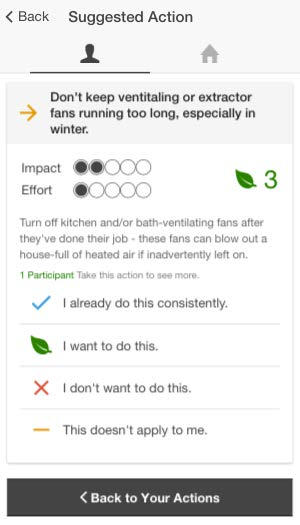
\includegraphics[width=0.3\linewidth]{img/action_details}
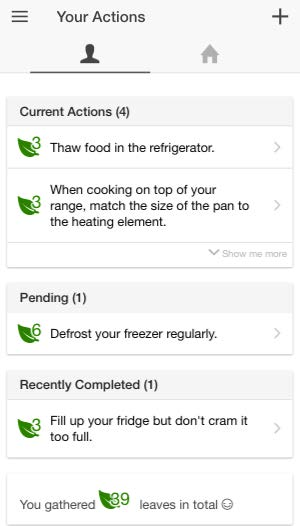
\includegraphics[width=0.3\linewidth]{img/action_tab}
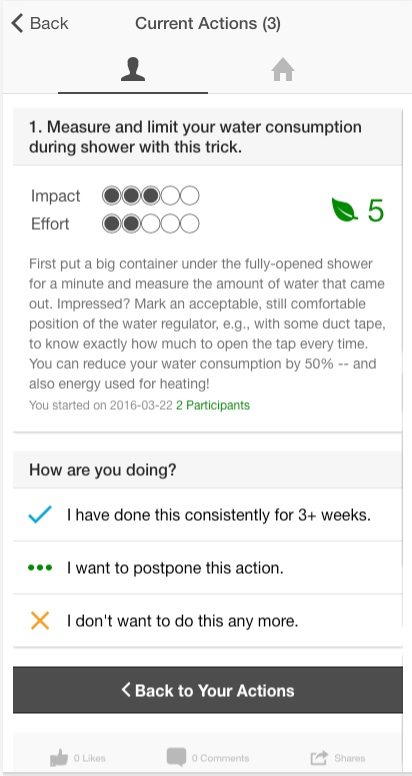
\includegraphics[width=0.279\linewidth]{img/Your_Actions.jpg}
\caption{(1) An action suggestion; (2) User actions tab; (3) An action in progress
}
\label{fig:actions}
\end{figure} 

\subsection{Fostering Motivation: Choosing Actions and Following the Behavior Change Process} 
\label{sec:example:motivation}

The action suggestions are not meant as prescriptions for what users should do but to present users different ideas of what they can do for energy conservation and how to do them in common household practices. The users are offered with a pool of suggestions which they can freely choose from and to follow according to their own everyday life context. Co-designed with local users (focus groups) and stakeholders, this line of thought is reflected in the design features of the application integrating the five design elements of the second design construct (Section~\ref{sec:motivation}).  


\subsubsection{Description of Key Features}
\label{sec:example:motivation:features}

With YouPower, a user can create a local project account or sign up with a Facebook account. A registered user can follow and practice a few self-selected energy conservation actions at a time. Each user has a self-configured personal and household profile, and an overview (the \textit{Your Actions} tab) of his/her own current, pending, and recently completed actions. Fig.~\ref{fig:actions}-(2) shows an example. 

A new/next action suggestion is presented to the user when an old/previous action is completed, or when the user wishes to add an action (by clicking an \textit{Add Action} button). When prompted with a suggestion, the user can decide whether to take the action, or indicate that he/she is alreading doing it or the suggestion is not applicable to his/her situation. Fig.~\ref{fig:actions}-(1) shows an example of four options: I already do this consistently; I want to do this; I don't want to do this; this doesn't not apply to me. 

Beside the information about an action itself (see Section~\ref{sec:example:suggestions}), the user is also presented with the information about how many users have been taking the action (including Facebook friends when logged in through Facebook). Each action has points (displayed as \textit{Green Leaves}) associated to the effort and impact score of that action. If the user completes an action, the leaves are awarded. 

After a suggested action is accepted, the user may also postpone (i.e. reschedule), abandon or indicate that the action is completed. Fig.~\ref{fig:actions}-(3) shows an example of three options: I have done this consistently; I want to postpone this action; I don't want to do this anymore. When an action is scheduled, e.g. \textit{defrost your fridge in $x$ days} ($x$ is set by a user), it will be triggered by time so that the application reminds the user of the pending action. In application settings, the user can also choose whether to repeat a completed action, reconsider a declined action, or reassess if an action is applicable to the user. 

After the user completes or abandons an action, YouPower asks feedback (to the project team). Fig.~\ref{fig:form} shows examples. The user is awarded with leaves if he/she gives comments and feedback (1 leaf each). 

\begin{figure}[t!]
      \begin{center}
        \begin{minipage}[t!]{0.3\linewidth}
	       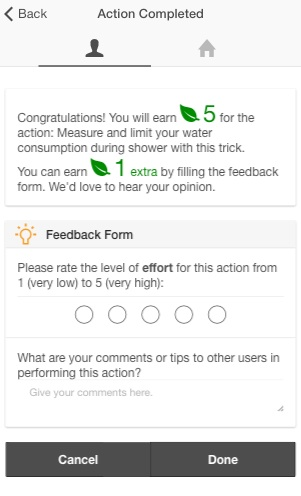
\includegraphics[width=1\linewidth]{img/action_completed.jpg}
           \vspace{1.95cm}
        \end{minipage}
        %\hfill 
        \begin{minipage}[t!]{0.3\linewidth}    
         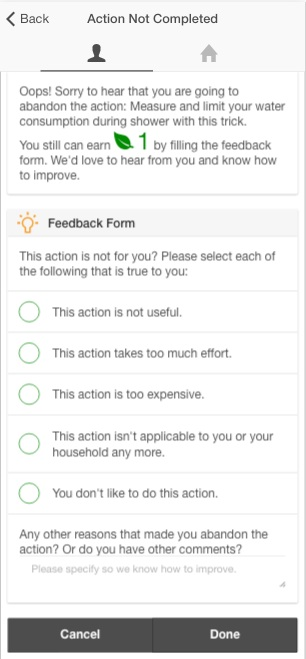
\includegraphics[width=1\linewidth]{img/action_not_completed.jpg}    
        \end{minipage}
      \end{center}
      \caption{Feedback form when a user (1) completes, or (2) abandons an action}\label{fig:form}
\end{figure}

YouPower encourages users to take small action steps and gives them positive performance feedback. For example, when a user is taking up many actions, the application can prompt that \textit{You already have $x$ actions in progress. You can add more actions after some of those are completed. Keep on! You are doing great.} 

A user can send email invitations to ask friends, family members, etc. to join YouPower (Fig.~\ref{fig:invite}). Family members can be added to a user's household,Fig.\ref{fig:house}-(1). If so, the user can see the actions of household members, Fig.\ref{fig:house}-(1), and add the actions to one's own action list. YouPower also supports popular social features such as \textit{Like} (with a \textit{Like} button) and commenting (on the actions). If logged in with a Facebook account, the user can ``share'' an action on Facebook. Fig.\ref{fig:share} shows an example.

\begin{figure}[h!]
      \begin{center}
        \begin{minipage}[t!]{0.3\linewidth}
	       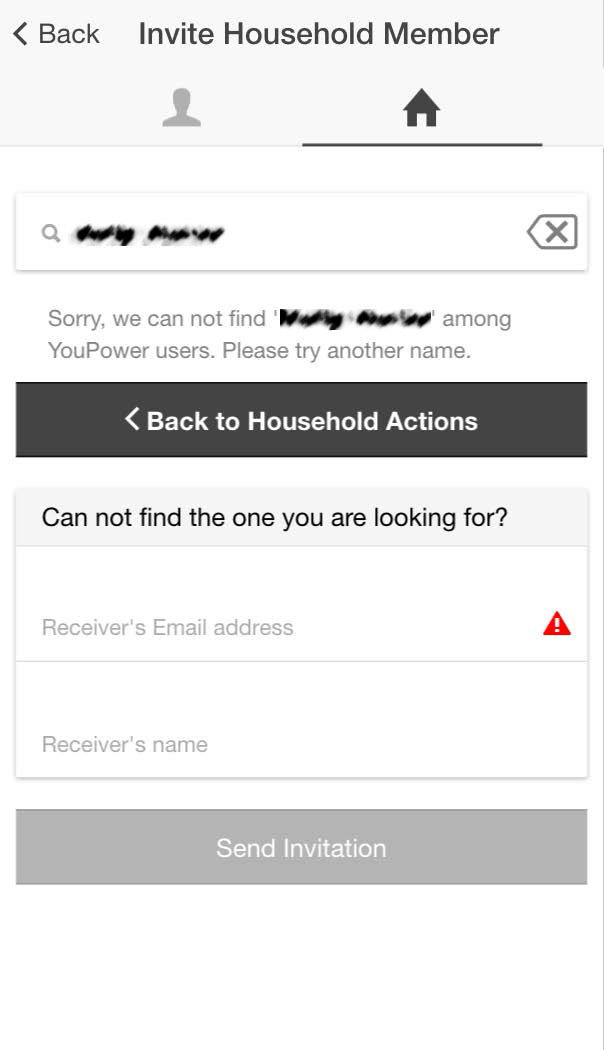
\includegraphics[width=1\linewidth]{img/invite1.jpg}
        \end{minipage}
        %\hfill 
        \begin{minipage}[t!]{0.6\linewidth}    
         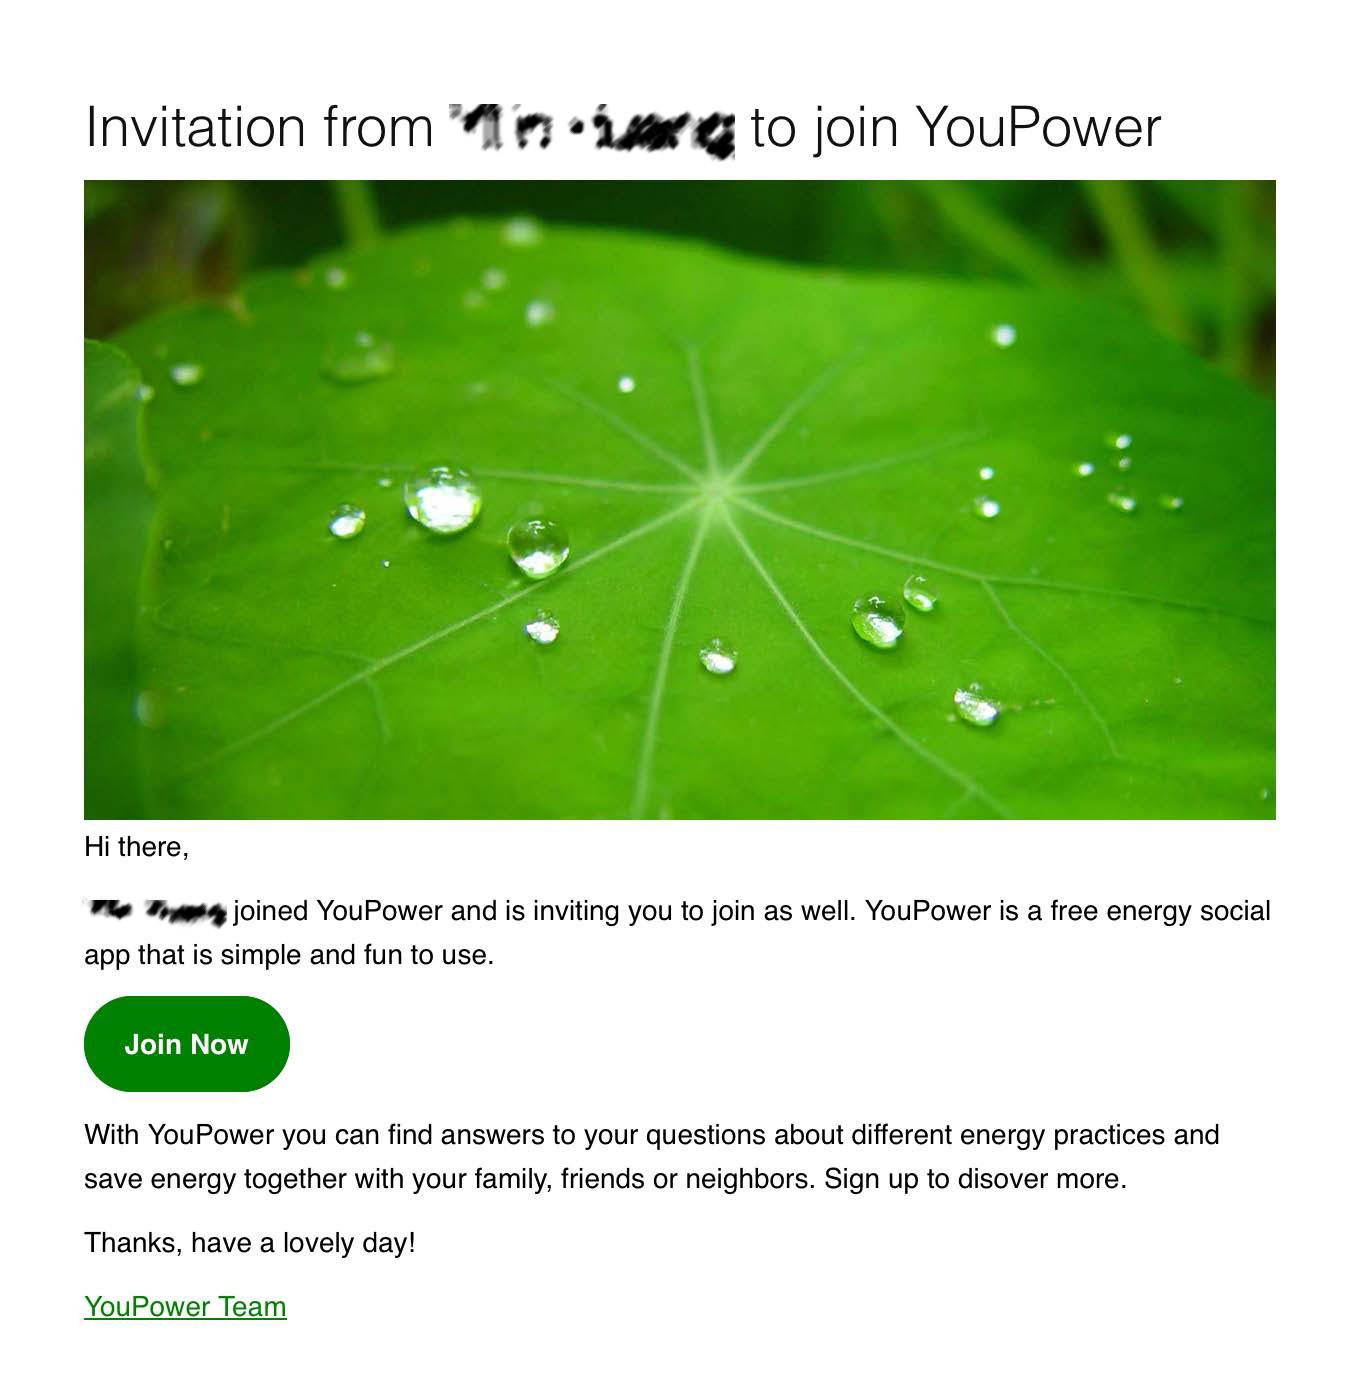
\includegraphics[width=1\linewidth]{img/invite2.jpg}    
        \end{minipage}
      \end{center}\caption{Send Email invitation to join YouPower }\label{fig:invite}
\end{figure}

\begin{figure}[t!]
      \begin{center}
        \begin{minipage}[t!]{0.3\linewidth}
	       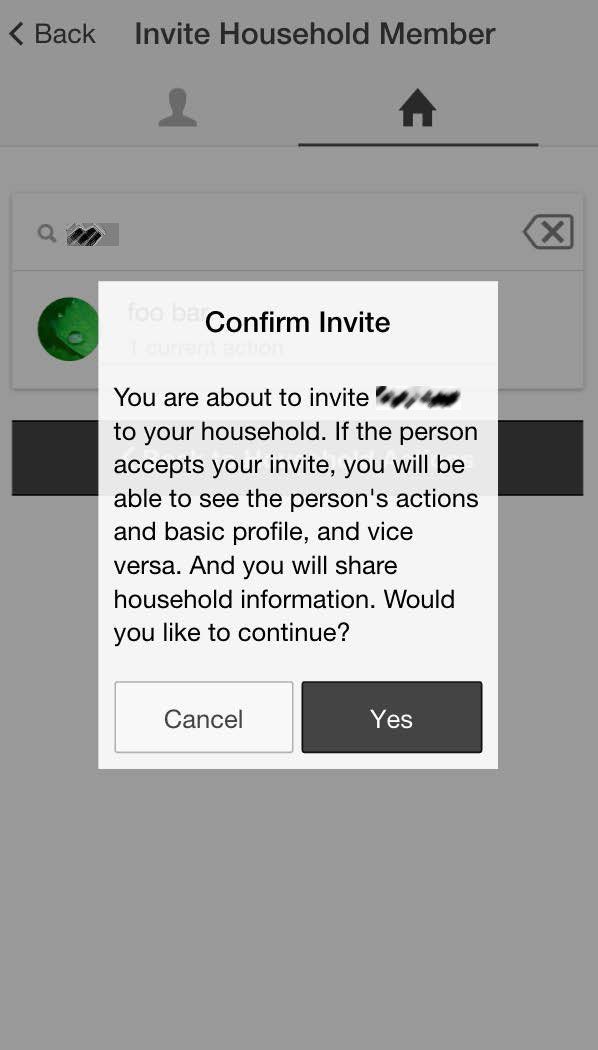
\includegraphics[width=1\linewidth]{img/house1.jpg}
        \end{minipage}
        %\hfill 
        \begin{minipage}[t!]{0.3\linewidth}    
         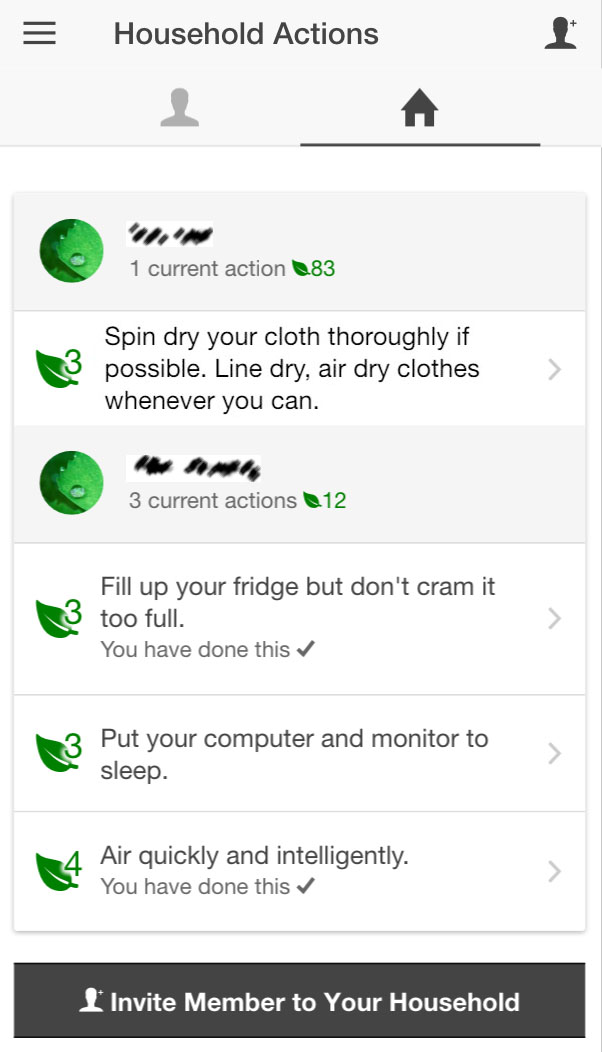
\includegraphics[width=1\linewidth]{img/house2.jpg}    
        \end{minipage}
      \end{center}
      \caption{(1) Invite household member; (2) Household member actions}\label{fig:house}
\end{figure}


\begin{figure}[t!]
\centering
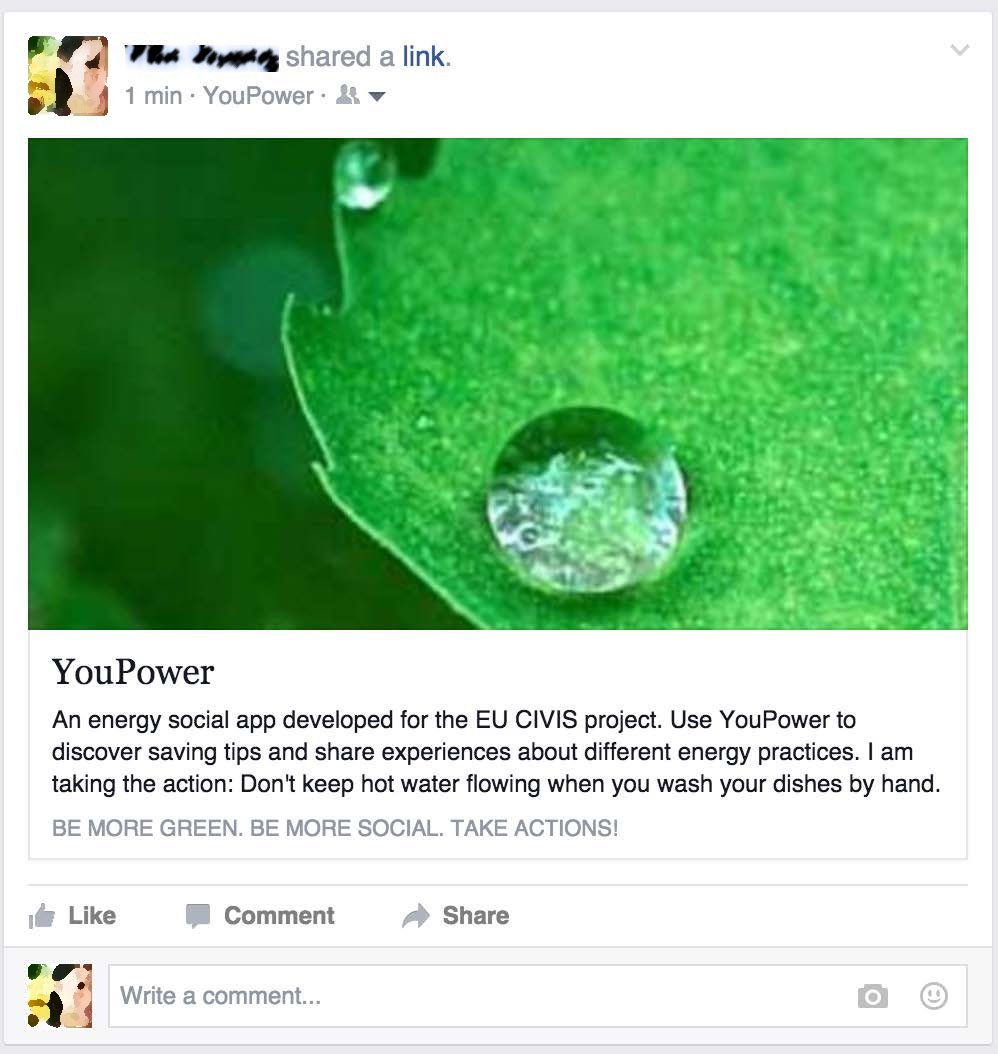
\includegraphics[width=0.55\linewidth]{img/share}
\caption{Facebook share of a YouPower action}
\label{fig:share}
\end{figure}

\subsubsection{Discussions} 
\label{sec:example:motivation:discussions}

To promote users' motivation and engagement in the behavior change process, a number of features address the design elements, providing support for competence, autonomy and self-reflection, and promoting altruistic and environmental values. They can be highlighted as follows.

For the options of choosing actions, first person narrative (e.g. \textit{I don't want to do this}) is used to create a personal micro-environment for the user \citep{Crumlish2009} to allow for a moment of self-reflection on one's own everyday energy practices, e.g. \textit{Does this action make sense to me (and my household)? Have I been indeed doing this? Do I want to do this?} By doing so, the user can identify whether an action is feasible in her/his own context, whether he/she has an attitude-behavior gap with regard to that particular action, if he/she feels competent in performing that action, and if so should he/she (and would he/she like to) change it. Similar design is use for completing/ rescheduling/ abandoning of actions. 

Such design allows users to freely choose whether (and when) to take an action or a series of actions, and to reschedule and repeat the actions according to their own everyday household practices. After all, users are experts of their own reality. By making such choices as revocable self-commitments, users themselves select actions that they are competent of doing in their everyday context, and they can adapt and follow the process of action-taking at a pace that suits their situations. The users also have free choices whether to give feedback and invite household members or new users, etc. These features facilitate the sense of competence and autonomy which promotes and enhances motivation. In addition, the users' choices, e.g. the commitment to an action, the completion or cancellation of an action, together with the other user inputs such as comments and feedback, etc., make a good data source for further research and personalization of the content. 

For the framing of the action suggestions, feedback forms, and other parts of the YouPower interface such as prompt messages, we carefully choose expressions and use \textit{Green Leaves} to promote altruistic and environmental values. The social features such as \textit{Like, Comment, Share} add social dynamics among users who can share and discuss their experiences and reflections with others. 

With an in-context email form, a user can send sign up invitations to friends, family members, etc. The altruistic and environmental values of joining and participating in YouPower are clearly articulated to the recipient in the email with a ``call to action'' \citep{Crumlish2009} button. The user can also send household member invitations and act upon them after receipt of such invitations. By adding household members, users can have an overview of the household actions. The design promotes household members to share the responsibility. Household energy conservation needs joint efforts. 

\section{Conclusion}
\label{sec:conclusion}

This paper calls for an approach to facilitate the behavior change process that is implementable in the context of one's everyday life as a key to address the attitude-behavior gap in household energy conservation. It is motivated by the fact that durable behavior change for energy conservation does not occur as a single event but rather as a gradual process, during which the context-specific reasons in people's everyday life have strong and immediate influences on specific actions, and the negative consequence of the constraints is often underestimated. For people who are willing to adopt ``green'' lifestyles but are constrained by the busyness and competing priorities of everyday practices, the facilitation of the behavior change process becomes an enabler in bridging the attitude-behavior gap. 

In this regard, two interrelated design constructs are proposed and discussed, namely (1) providing consumers accurate information about actionable suggestions in the specific context of their everyday life, and (2) fostering consumers' motivation to engage in the behavior change process towards energy conservation. The design suggestions aim to enable and encourage energy conservation integrated into people's everyday life without being in conflict with their primary goals and everyday needs so as to produce sustained behavior change. This line of thought in design is exemplified by YouPower, a hybrid mobile application designed to provide easy access for users to adapt and follow up the process of voluntary behavior change in the busyness and competing priorities of their everyday life.

This paper does not intend to suggest that facilitating the behavior change process is the solution to the attitude-behavior gap in household energy conservation. There is no silver bullet in the form of a single theory, method, approach or application that guarantees to address the attitude-behavior gap in energy conservation and environmental issues in large. Since energy consumption behavior in everyday life is a complex open system and people by themselves are inherently different, it is arguably neither feasible nor useful to define general rules that incorporate all factors that influence people's energy conservation behavior. Given that some behavior intervention strategies can be effective for some people in some context, it is vital for interventions to be exploratory and adaptive trying out multiple methods and different approaches that could be potentially fruitful for different people in achieving the goal. 

Our future research will follow through the proposed approach in the test sites deployment and its effect in the long term. Future research can also explore structural intervention strategies (\cite{Steg2008}, i.e. strategies that focus on altering the context in which action decisions are made so as to make energy conservation more attractive) in the direction of facilitating the behavior change process. 

%\renewcommand{\bibfont}{\small}
\printbibliography

\end{document}

